
\documentclass{beamer}

%\usepackage[table]{xcolor}
\mode<presentation> {
  \usetheme{Boadilla}

%  \usetheme{Pittsburgh}
%\usefonttheme[2]{sans}
\renewcommand{\familydefault}{cmss}
%\usepackage{lmodern}
%\usepackage[T1]{fontenc}
%\usepackage{palatino}
%\usepackage{cmbright}
  \setbeamercovered{transparent}
\useinnertheme{rectangles}
}

\setbeamercolor{normal text}{fg=black}
\setbeamercolor{structure}{fg= blue}
\definecolor{trial}{cmyk}{1,0,0, 0}
\definecolor{trial2}{cmyk}{0.00,0,1, 0}
\definecolor{darkgreen}{rgb}{0,.4, 0.1}
\usepackage{array}
\beamertemplatesolidbackgroundcolor{white}  \setbeamercolor{alerted
text}{fg=red}
\usepackage{tcolorbox}
\setbeamertemplate{caption}[numbered]\newcounter{mylastframe}


\usepackage{tikz}
\usetikzlibrary{arrows}
\usepackage{colortbl}

\renewcommand{\familydefault}{cmss}
%\usepackage[all]{xy}

\usepackage{tikz}
\usepackage{lipsum}

 \newenvironment{changemargin}[3]{%
 \begin{list}{}{%
 \setlength{\topsep}{0pt}%
 \setlength{\leftmargin}{#1}%
 \setlength{\rightmargin}{#2}%
 \setlength{\topmargin}{#3}%
 \setlength{\listparindent}{\parindent}%
 \setlength{\itemindent}{\parindent}%
 \setlength{\parsep}{\parskip}%
 }%
\item[]}{\end{list}}
\usetikzlibrary{arrows}

\usecolortheme{lily}

\newtheorem{com}{Comment}
\newtheorem{lem} {Lemma}
\newtheorem{prop}{Proposition}
\newtheorem{condition}{Condition}
\newtheorem{thm}{Theorem}
\newtheorem{defn}{Definition}
\newtheorem{cor}{Corollary}
\newtheorem{obs}{Observation}
 \numberwithin{equation}{section}
 

\setbeamertemplate{navigation symbols}{}


\title[PLSC 43401]{Mathematical Foundations of Political Methodology}

\author{Robert Gulotty}
\institute[Chicago]{University of Chicago}
\vspace{0.3in}




\begin{document}

\begin{frame}
\maketitle
\end{frame}


\begin{frame}
\frametitle{Confidence intervals}
\begin{itemize}
\item Interval Estimation
\item Hypothesis Testing
\item Power and Confidence
\item P values
\end{itemize}
\end{frame}



\begin{frame}{Interval Estimation}
\begin{itemize}
\item An interval estimator maps a random variable onto an interval, rather than a point.\pause
\item If our estimator is $\hat{\theta}$, an interval estimator is written 
$$[\hat{\theta}_{lower},\ \hat{\theta}_{upper}]$$\pause
\item The interval represents the range of possible values within which we are confident to find the true $\theta$. \pause
\item This is often called a confidence interval.
\end{itemize}
\end{frame}



\begin{frame}{Interval Estimation}
\begin{defn}
A confidence interval with a confidence level $1-\alpha$ is an interval estimator $[\hat{\theta}_{lower},\ \hat{\theta}_{upper}]$, that is guaranteed to cover the true parameter $100\times (1-\alpha)$ of the time.\pause
\end{defn}
\begin{itemize}
\item Coverage probability describes how likely it is that the interval covers the true parameter value.\pause
\item Shorter intervals are better.
\end{itemize}
\end{frame}



\begin{frame}{Normal Population with known $\sigma^2$}
\begin{itemize}
\item Suppose we have $n$ draws from a Normal distribution $N(\mu,\ 2)$

$$\frac{\bar{X}_n-\mu}{2/\sqrt{n}}\sim N(0,1)$$\pause
\item Using the inference from before,\pause
$$F(1.96)=P(\frac{|\bar{X}_n-\mu|}{2/\sqrt{n}}<1.96)=.95 $$\pause
$$P(-1.96<\frac{\bar{X}_n-\mu}{2/\sqrt{n}}<1.96)=.95$$
\end{itemize}
\end{frame}


\begin{frame}{Normal Population with known $\sigma^2$}
\begin{itemize}
\item A confidence interval is just a rearrangement:
$$P(-1.96<\frac{\bar{X}_n-\mu}{2/\sqrt{n}}<1.96)=.95$$\pause
$$P(-1.96*2/\sqrt{n}<\bar{X}_n-\mu<1.96*2/\sqrt{n})=.95$$\pause
$$P(\bar{X}_n-1.96*2/\sqrt{n}<\mu<\bar{X}_n+1.96*2/\sqrt{n})=.95$$\pause
\item So the following interval estimator contains the true population $\mu$ with probability .95:
$$[\bar{X}_n-1.96*2/\sqrt{n}, \bar{X}_n+1.96*2/\sqrt{n}]$$

\end{itemize}
\end{frame}

\begin{frame}[fragile]{Simulations}
\begin{verbatim}
> library(animation)
> conf.int()
\end{verbatim}
\end{frame}



\begin{frame}{Example Normal Population with known $\sigma^2$}
\begin{itemize}
\item Suppose that the WHO is enacting a new Ebola monitoring service at 400 airports which may hold up lines. \pause
\item Suppose that we know that the ebola monitoring service has historically had a variance of  9 people per hour and is normally distributed. \pause
\item We surveyed 40 of these monitors, and found that the sample had an average speed of 70 people per hour.\pause
\item What is the estimate of the speed of the service?\pause
\item The following interval \alert{estimator} contains the true population $\mu$ with probability .95:
$$[\bar{X}_n-1.96*\sigma/\sqrt{n}, \bar{X}_n+1.96*\sigma/\sqrt{n}]$$\pause
\item The following interval \alert{estimate} has a confidence level of .95:
$$[70-1.96*3/\sqrt{40}, 70+1.96*3/\sqrt{40}]$$

\end{itemize}
\end{frame}

\begin{frame}{The shortest interval}
\begin{itemize}
\item If $\hat{\theta}\sim N(\mu, \sigma)$
$$[\hat{\theta}-z_{\alpha/2} *\sqrt{var(\hat{\theta})},\ \hat{\theta}+z_{\alpha/2}*\sqrt{var(\hat{\theta})}]$$\pause
\item If $\hat{\theta}\sim t_{n-1}$
$$[\hat{\theta}-t_{n-1}(\alpha/2) *\sqrt{S^2}/\sqrt{n},\ \hat{\theta}+t_{n-1}(\alpha/2) *\sqrt{S^2}/\sqrt{n}]$$

\end{itemize}

\end{frame}


\begin{frame}{Example Normal Population with unknown $\sigma^2$}
\begin{itemize}
\item Suppose that we are trying to find the average height of a village in Afghanistan.\pause
\item Suppose that we know that altitude is normally distributed. \pause
\item We surveyed 20 villages, and found that the sample had an average altitude of 3200 meters with a sample variance of 1200 meters.\pause
\item What is the estimate of the average altitude in Afghanistan?\pause
\item We use the $t$ distribution with 19 degrees of freedom.
\item The following interval \alert{estimate} has a confidence level of .95:
$$[3200-t_{19}(\alpha/2) *\sqrt{1200)}/\sqrt{20},\ 3200+t_{19}(\alpha/2) *\sqrt{1200}/\sqrt{20}]$$\pause
$$[3200-2.09*\sqrt{1200)}/\sqrt{20},\ 3200+2.09 *\sqrt{1200}/\sqrt{20}]$$

\end{itemize}
\end{frame}

\begin{frame}{Interpretation}
\begin{itemize}
\item A 95\% confidence interval is an estimate of plausible values for the population parameter.  \pause
\item It is not a measure of the degree of probability, belief, or support that an unknown parameter value lies in \emph{this} specific interval. \pause 
\item A particular confidence interval of 95\%  does not mean that there is a 95\% probability of a sample mean from a repeat of the experiment falling within \emph{this} interval.
\item A 95\% confidence interval does not mean that 95\% of the sample data lie within \emph{this} interval.
\end{itemize}
\end{frame}

\begin{frame}{Confidence interval for the difference in means with known variances}
\begin{itemize}
\item Suppose that we are trying to find the average height of a village in Afghanistan relative to a village in Pakistan.\pause
\item Suppose that we know that altitude is normally distributed, and the variance is 1200 meters and 200 meters respectively. \pause
\item We surveyed 20 villages in Afghanistan and 30 villages in Pakistan, $\bar{X}_A= 3200$,$\bar{X}_P= 1200$ \pause
\item What is the estimate of the difference in average altitudes?\pause
\item The difference in Normals is normal.  $$\bar{X}_A-\bar{X}_P\sim N\left(\mu_A-\mu_P, \sqrt{(\frac{\sigma^2_A}{n_A}+\frac{\sigma^2_P}{n_P})}\right)$$
\item The following interval \alert{estimate} has a confidence level of .95:
$$[\bar{X}_A-\bar{X}_P-z_{\alpha/2} *\sqrt{(\frac{\sigma^2_X}{n_X}+\frac{\sigma^2_Y}{n_Y})},\ \bar{X}_A-\bar{X}_P+z_{\alpha/2}*\sqrt{(\frac{\sigma^2_X}{n_X}+\frac{\sigma^2_Y}{n_Y})}]$$


\end{itemize}
\end{frame}

\begin{frame}{Hypothesis Tests}
\begin{itemize}
\item Point estimation: what is the most likely value of the parameter?
\item Interval Estimation: what is the range of plausible values of the parameter?
\item Hypothesis testing: do we have evidence to reject a hypothesized interval of parameter values?
\item Failure to find such evidence does not suggest that the hypothesis is true.
\end{itemize}
\end{frame}


\begin{frame}{Definition of Hypothesis}
\begin{defn}
A \alert{hypothesis} is a statement about a population parameter
\end{defn}\pause
\begin{itemize}
\item Does democracy promotion promote peace? (lower rates of conflict among treatment group).\pause
\item Do treaties constrain countries? (is behavior distinct among treaty signers?)\pause
\item Is support for Trump above 50\%?\pause
\item Is Ohio State good this year?
\end{itemize}
\end{frame}



\begin{frame}{Definition of Hypothesis Test}
\begin{defn}
A \alert{Hypothesis Test} compares two mutually exclusive sets of parameters,
\begin{itemize}
\item Null hypothesis: $H_0$
\item Alternative hypothesis: $H_1$
\end{itemize}
\end{defn}\pause
\begin{itemize}
\item Does democracy promotion promote peace? \pause
\begin{itemize}
\item $H_0$: Democracy promotion does not promote peace (treated and untreated groups are equally conflictual).
\item $H_1$: Democracy promotion promotes peace (treated and untreated groups are different).
\end{itemize}
\item Is Ohio State good this year?
\begin{itemize}
\item $H_0$: Ohio State is good this year
\item $H_1$: Ohio State is not particularly good.
\end{itemize}
\end{itemize}
\end{frame}

\begin{frame}{Testing Procedure}
\begin{defn}
Given a test statistic t(X), a hypothesis testing procedure is a rule that specifies
\begin{itemize}
\item Value of test statistic when we do not reject $H_0$: acceptance region\pause
\item Value of test statistic when we do reject $H_0$: rejection region\pause
\item Value separating regions: critical value
\end{itemize}
\end{defn}
\end{frame}

\begin{frame}{Example: Homework times }
\begin{itemize}
\item I had a theory that students should study for 10 hours a week.\pause
\item Is that theory consistent with practice?\pause
\item $H_0:$ $\mu =10$ (The homework is fine.)\pause
\item $H_1:$ $\mu \neq 10$  (I should make more difficult or easier homework).
\item Failing to reject the null does not mean that the null is true.
\end{itemize}
\end{frame}

\begin{frame}{Example: Homework}
\begin{itemize}
\item We can estimate $S^2=\frac{1}{N-1}\sum_{i=1}^N(X_i-\bar{X})^2$\pause
$$\frac{\bar{X}-\mu}{S/\sqrt{N}}\sim t_{N-1}$$\pause
\item $\frac{\bar{X}-\mu}{S/\sqrt{N}}$ is our test statistic. \pause
\item Assume that the null hypothesis is true, plug in for $\mu$
\end{itemize}
\end{frame}


\begin{frame}{Error Types}
\begin{table}[htdp]
\begin{center}
\begin{tabular}{l|c|c|}
& Fail to Reject $H_0$& Reject $H_0$\\
\hline
$H_0$ True& Correct & Type I Error\\
$H_1$ True& Type II Error & Correct\\
\end{tabular}
\end{center}
\end{table}
\begin{itemize}
\item Type I Error: reject a null that is true\pause
\item[] Deciding the homework is too hard when it is not.\pause
\item Type II Error: failing to reject a null that is false.\pause
\item[] Leaving the homework the same when it is too hard.\pause
\end{itemize}
The \alert{Size} of test ($\alpha$) is the probability of Type I Error (false discovery).\\ \pause
The \alert{Power} of test is 1 - the probability of Type II Error ($\beta$) (failed discovery).\\
What is worse: False discovery or missed detection?\\\pause
What is worse: me having to make homework easier or you having to suffer from continued hard homework.
\end{frame}


\begin{frame}{Example of Test Statistic and Critical Region}
\begin{itemize}
\item Set $\mu=10$\pause
\item $t(X)\equiv \frac{\bar{X}-10}{s/\sqrt{N}}\sim t_{N-1}$\pause
\item Critical value ($x_0$): how long would you have to take on average for me to feel that you are working too hard?\pause
\item $P(|t(X)|>x_0)=\alpha$\pause
\item $P(t(X)< -x_0)+P(t(X)> x_0)=\alpha$
\item $P(t(X)>x_0)=\alpha/2$
\end{itemize}
\end{frame}


\begin{frame}{Example of Test Statistic and Critical Region}
\begin{itemize}
\item Set $\mu=10$ for 22 students.\pause
\item Set $\alpha=.05$\pause
\item Using the t distribution, $x_0$ is $2.07$\pause
\item Suppose the sample mean is 12 hours.\pause
\item Suppose the sample standard deviation is 2.6 hours.
$$P(t(X)>x_0)$$\pause
$$\frac{12-10}{2.6/\sqrt{22}}>2.07$$
$$3.6>2.07$$\pause
$$\text{p-value}=\int_{t(X)}^\infty f(x)dx=0.0008$$
\end{itemize}
\end{frame}



\begin{frame}[plain]
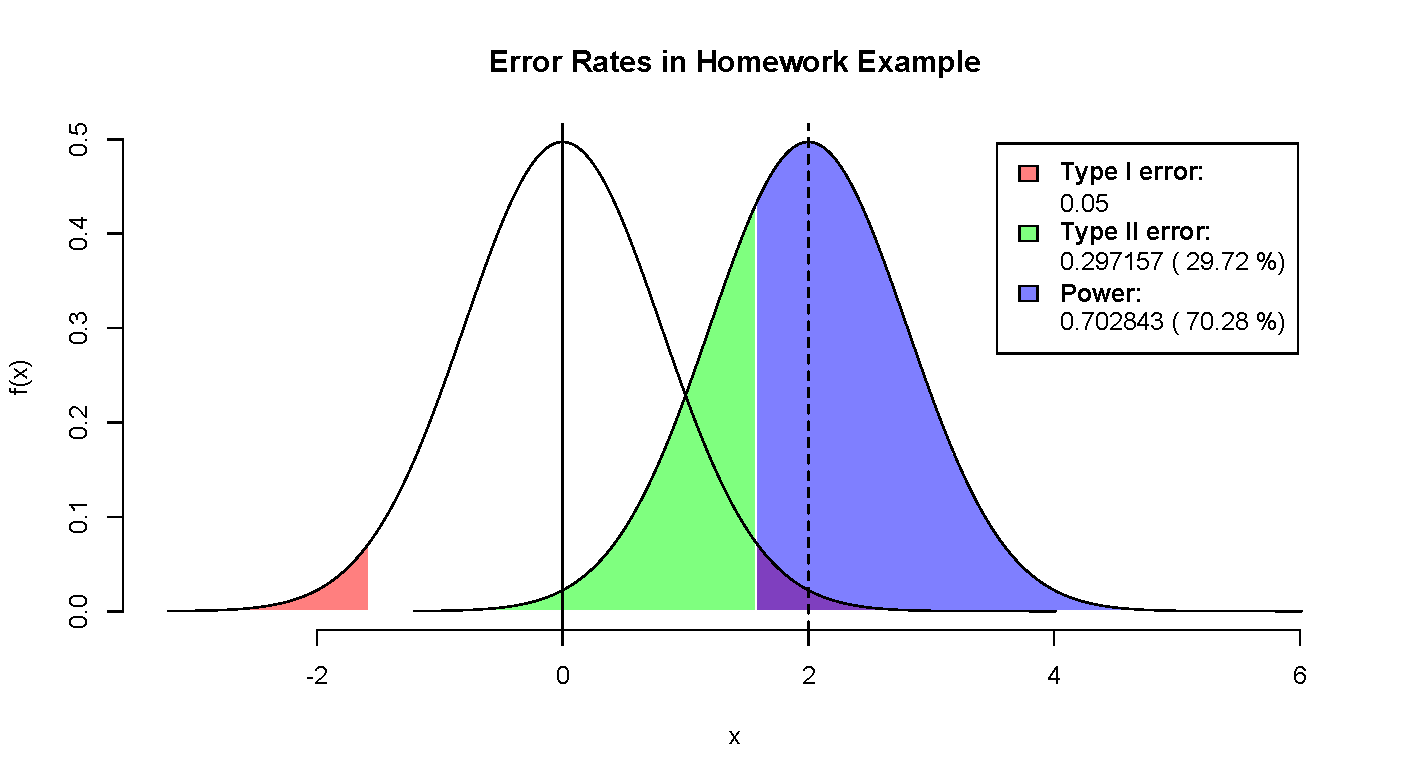
\includegraphics[width=4 in]{VisualizationHomework.pdf}

\end{frame}


\begin{frame}[plain]{Increase $\alpha$}
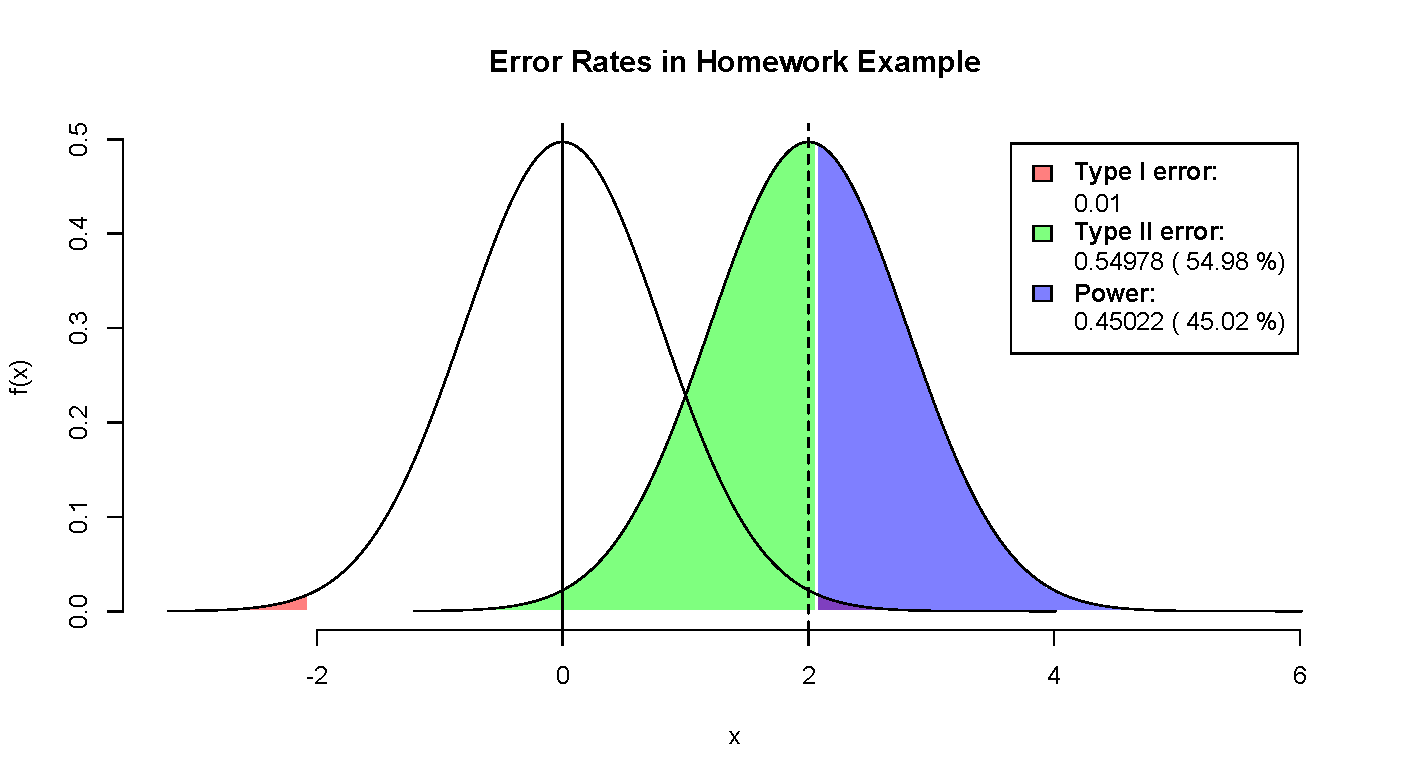
\includegraphics[width=4 in]{VisualizationHomework2.pdf}

\end{frame}


\begin{frame}[plain]
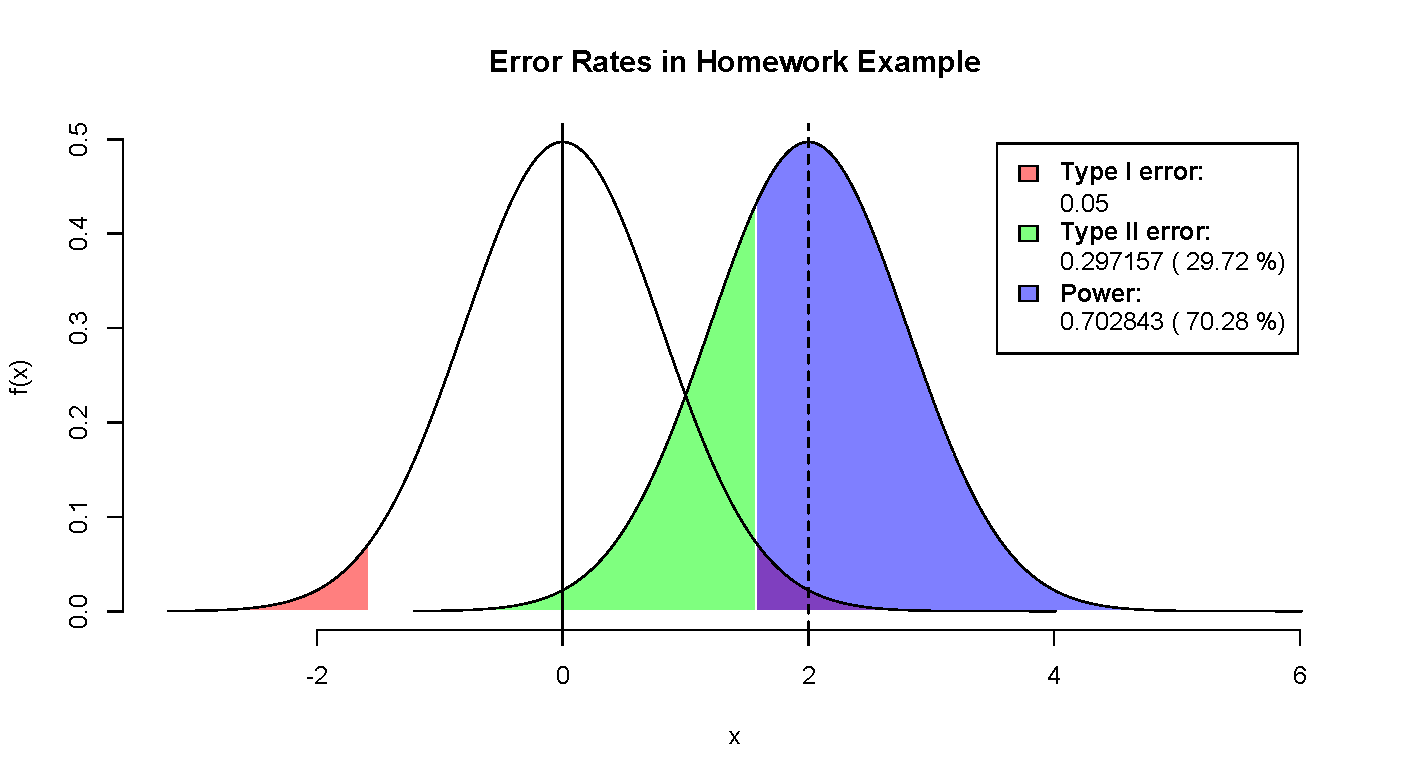
\includegraphics[width=4 in]{VisualizationHomework.pdf}

\end{frame}


\begin{frame}[plain]{Triple sample size}
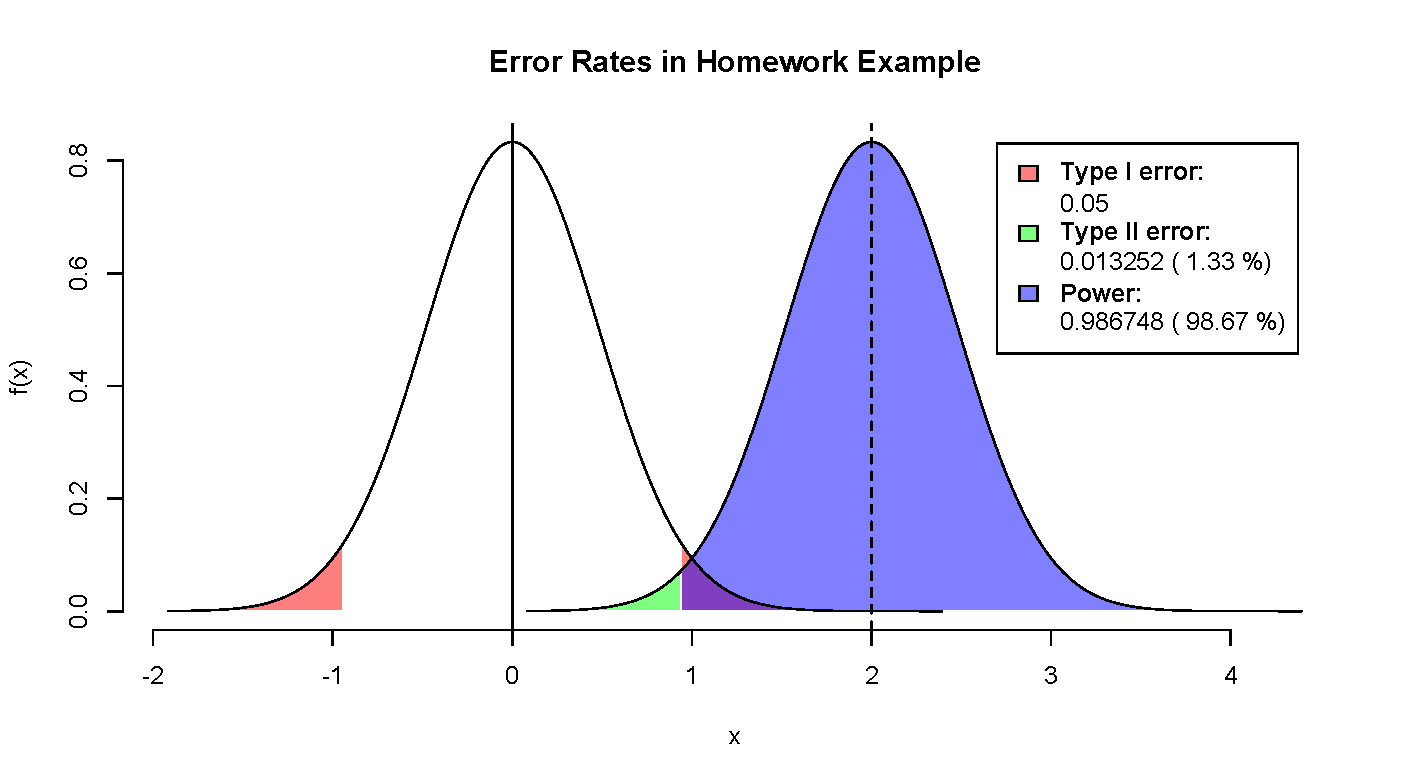
\includegraphics[width=4 in]{VisualizationHomework3.pdf}

\end{frame}

\begin{frame}[plain]
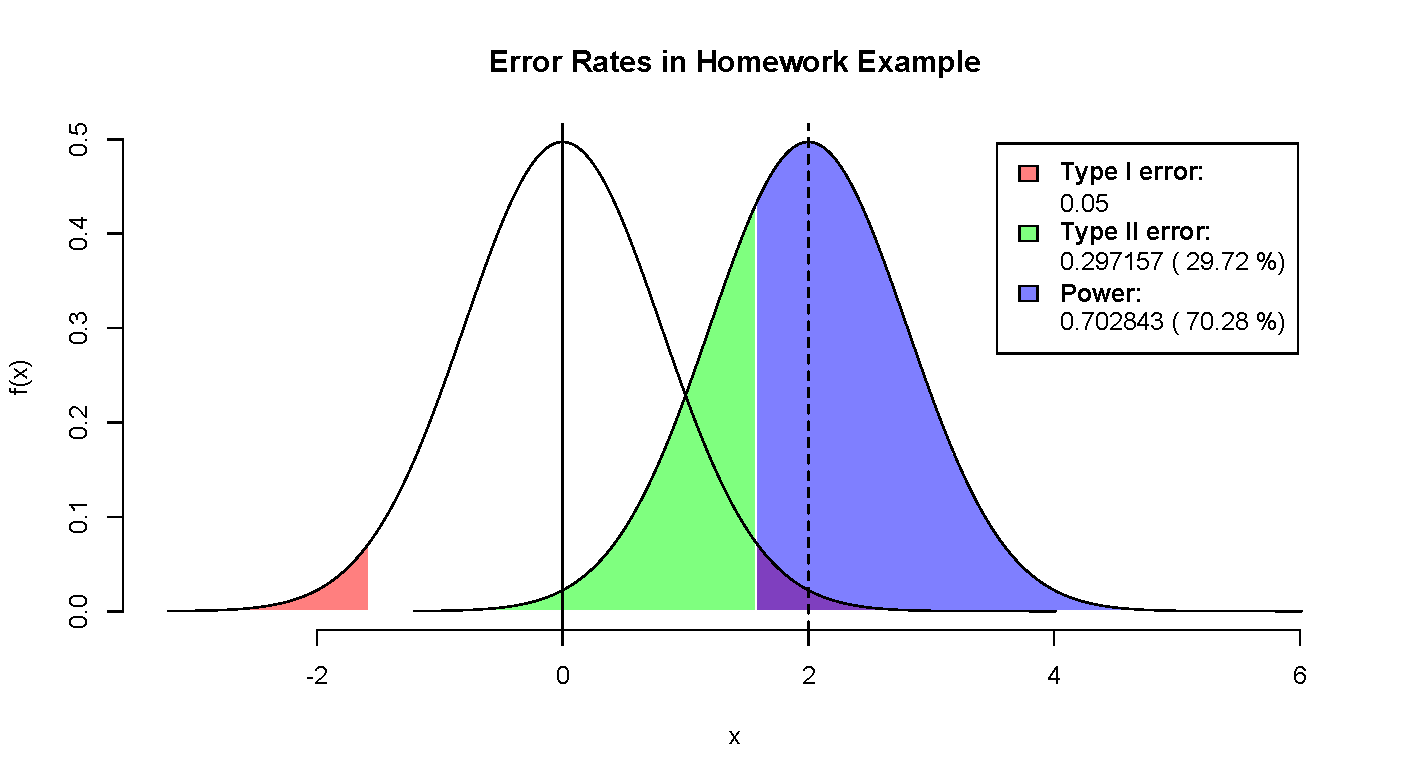
\includegraphics[width=4 in]{VisualizationHomework.pdf}

\end{frame}


\begin{frame}[plain]{Decrease $\sigma$}
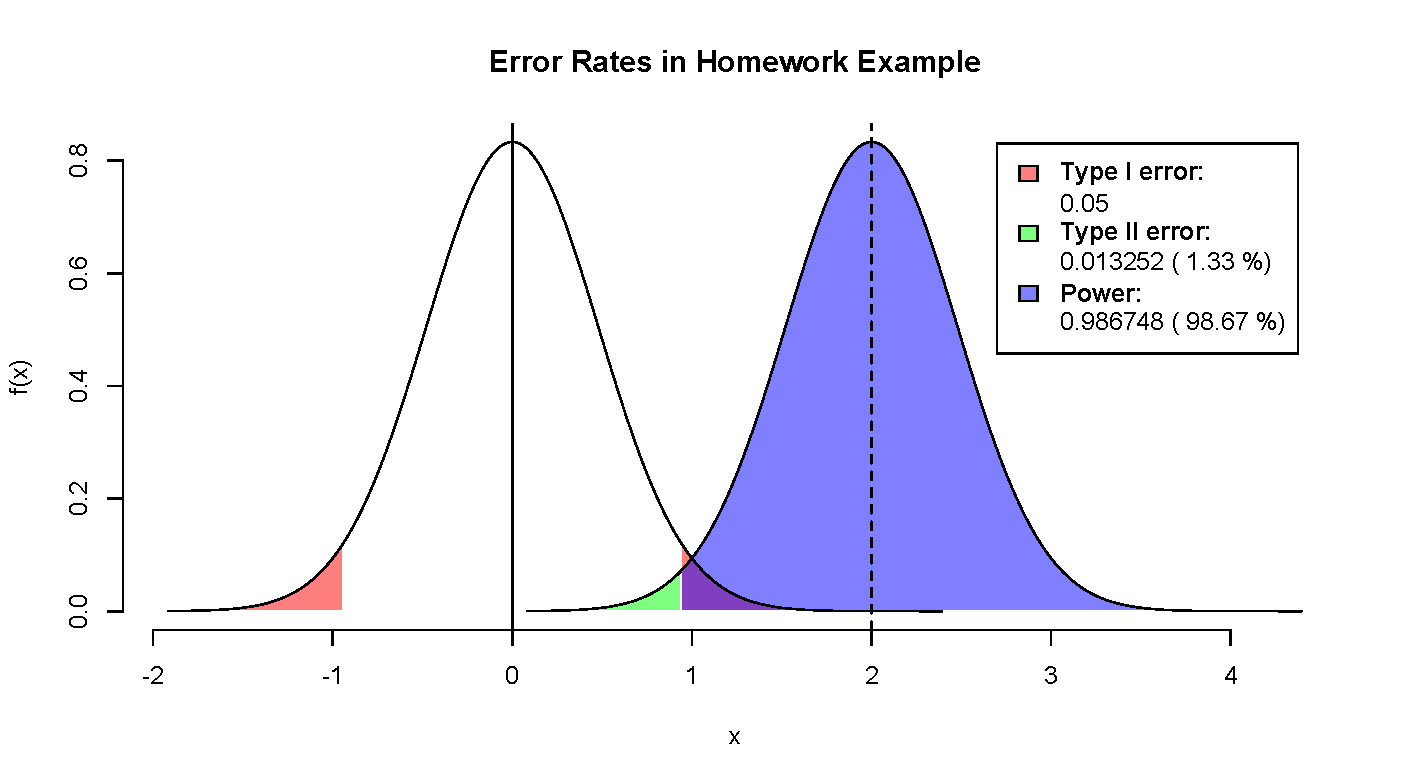
\includegraphics[width=4 in]{VisualizationHomework3.pdf}

\end{frame}

\begin{frame}{Summary}

Power will depend on four factors:
\begin{itemize}
\item Effect size
\item Size of test $\alpha$
\item Sample size
\item $\sigma^2$\pause
\end{itemize}
Failing to reject the null does not mean that the null is true.
\end{frame}

\begin{frame}{Confidence Intervals and Hypothesis testing.}
\begin{itemize}
\item If $\hat{\theta}\sim N(\mu, \sigma)$, the confidence intervals are:
$$[\hat{\theta}-z_{\alpha/2} *\sqrt{var(\hat{\theta})},\ \hat{\theta}+z_{\alpha/2}*\sqrt{var(\hat{\theta})}]$$\pause
\item If $\hat{\theta} = \hat{\theta}_1-\hat{\theta}_0\sim N(\mu, \sigma)$, the rejection region is:
$$(-\infty, \hat{\theta}-z_{\alpha/2} *\sqrt{var(\hat{\theta})}]\cup [\hat{\theta}+z_{\alpha/2}*\sqrt{var(\hat{\theta})}, \infty)$$\pause
\item Confidence intervals cover all null hypotheses we would fail to reject.\pause
\item Failing to reject the null does not mean that the null is true.
\end{itemize}
\end{frame}

\begin{frame}
A p-value p(X) is a test statistic which gives a continuous evaluation of a hypothesis.  The smaller the p-value, the stronger the evidence for rejecting the null hypothesis.\pause

If $X_1,\ X_2,\ X_3,\ldots X_n$  is a random sample from a $N(\mu \sigma^2)$ data, $\frac{\bar{X}-\mu_0}{S/\sqrt{n}}$ has a students t distribution with $n-1$ degrees of freedom.

$$p(x)=2*P(T_{n-1} \geq \frac{|\bar{x}-\mu_0|}{(s/\sqrt{n})})$$\pause

$$p(x)=2*(1-\texttt{pt}(\frac{|\bar{x}-\mu_0|}{(s/\sqrt{n})},\ n-1))$$

\end{frame}




\begin{frame}{P values}
\begin{itemize}
\item P-values tell us how likely the data is if the null hypothesis were true.  \pause
\item People like to use p values to print *** in their papers.
\item Failing to reject the null does not mean that the null is true. In fact we assume it is true to calculate the p-value.\pause
\item We usually do not care about the null hypothesis, we care about our favorite hypothesis.\pause
\item P-values do not tell us how certain we are about a result.
\end{itemize}
\end{frame}


\begin{frame}{More Cautionary notes}
\begin{itemize}
\item  A statistically significant finding is not necessarily evidence of something substantively important.\pause
\item Studies will have different p-values by chance.  \pause
\item $P=.05$ tells us that 5\% of the time we would see data \alert{at least} as weird as this if the null hypothesis were true.\pause
\item You should generally not base decisions on whether or not your p-value takes on a certain value.
\end{itemize}
\end{frame}

\begin{frame}{What to do?}
\begin{itemize}
\item Report more information about the distribution.
\item Design studies so that you care about the estimates, not just rejecting a null hypothesis.
\end{itemize}
\end{frame}

\end{document}